% https://latexdraw.com/how-to-highlight-parts-of-a-function-and-change-the-background-color-in-latex-using-tikz/
% arr: indenting code; add comments
\documentclass[dvipsnames]{standalone}

\usepackage{tikz}
\usepackage{pgfplots}
\pgfplotsset{compat = newest}

\begin{document}
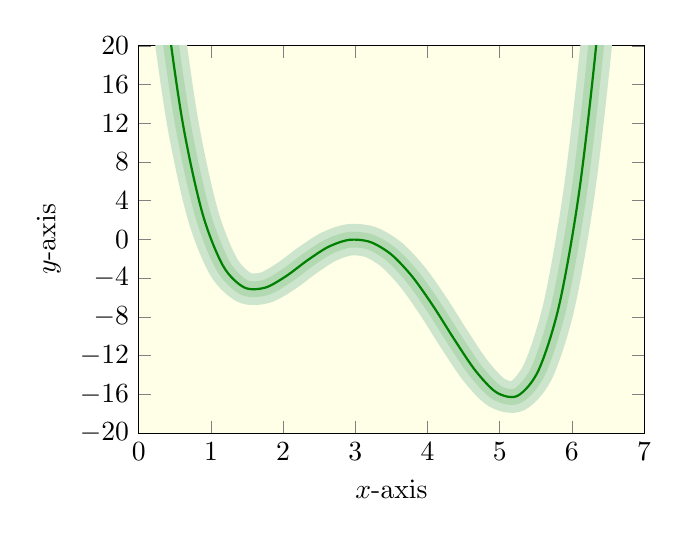
\begin{tikzpicture}
	\begin{axis}
		[
			xmin = 0, xmax = 7,
			ymin = -20, ymax = 20,
			width = 8cm,
			height = 6.5cm,
			xtick distance = 1,
			ytick distance = 4,
			smooth,
			xlabel=$x$-axis,
			ylabel=$y$-axis,
			set layers,
		]
		% plot background yellowish
		\begin{pgfonlayer}{axis background}
			\fill [yellow!10] (0,-20) rectangle (7,20);
		\end{pgfonlayer}
		% superposing three curves with different thickness and colors
		\addplot[Green!20, domain = 0:7, line width=4mm] {(x-1)*(x-3)^2*(x-6)};   % very thick curve
		\addplot[Green!30, domain = 0:7, line width=2mm] {(x-1)*(x-3)^2*(x-6)}; % thick curve
		\addplot[Green, domain = 0:7, thick] {(x-1)*(x-3)^2*(x-6)};             % thin curve
	\end{axis}

\end{tikzpicture}
\end{document}